% This is samplepaper.tex, a sample chapter demonstrating the
% LLNCS macro package for Springer Computer Science proceedings;
% Version 2.20 of 2017/10/04
%
\documentclass[runningheads]{llncs}
%
\usepackage{graphicx}
% Used for displaying a sample figure. If possible, figure files should
% be included in EPS format.
%
% If you use the hyperref package, please uncomment the following line
% to display URLs in blue roman font according to Springer's eBook style:
% \renewcommand\UrlFont{\color{blue}\rmfamily}

% listings
\usepackage{xcolor,listings}
\usepackage{textcomp}
\lstset{upquote=true}

\begin{document}
%
\title{Calco: Contract-based Approach\\ to Specify Dataflows}
%
%\titlerunning{Abbreviated paper title}
% If the paper title is too long for the running head, you can set
% an abbreviated paper title here
%
\author{Andrey Stoyan\inst{1} \and
Artem Trofimov\inst{1} \and
Nikita Sokolov\inst{1} \and
Boris Novikov\inst{2} \and
Igor E. Kuralenok\inst{1}}
%
\authorrunning{A. Stoyan et al.}
% First names are abbreviated in the running head.
% If there are more than two authors, 'et al.' is used.
%
\institute{Yandex \and
National Research University Higher School of Economics}
%
\maketitle              % typeset the header of the contribution
%
\begin{abstract}
    Distributed dataflows can be specified in two ways: by defining an execution graph or specifying the desired result, e.g., using SQL.
    An execution graph consists of arbitrary operations, so it cannot be automatically transformed for optimization.
    SQL is popular for data analytics, and its optimization is well-researched.
    However, it is sometimes inconvenient or impossible to use SQL for general data management tasks, such as ETL, machine learning pipelines, etc.
    In this work, we introduce a novel approach to specify distributed dataflows.
    Our method is based on declarative specifications of user-defined operations called contracts.
    Such specifications allow us to build a set of equivalent graphs, which form a space for optimization.
    We implement a graphs generation prototype and outline the challenges regarding the optimization problem.

\keywords{Optimization.}
\end{abstract}
%
%
%
\section{Introduction}
Distributed batch processing systems, such as Google MapReduce~\cite{Dean:2008:MSD:1327452.1327492}, Apache Hadoop~\cite{hadoop2009hadoop}, and Apache Spark~\cite{Zaharia:2016:ASU:3013530.2934664}, address the need to process large amounts of data (e.g., Internet-scale). The basic idea behind them is to independently process large data blocks (batches) that are collected from static datasets. The main advantages of these systems are the fault tolerance and scalability~\cite{borthakur2011apache} of massively parallel computations on commodity hardware. Batch processing ensures latency in terms of hours or even days~\cite{carbone2015apache, chang2014hawq, sun2023survey}. 

Batch processing is suitable for scenarios where data freshness is not a critical factor, such as in the collection of large datasets, exract-transform-load (ETL) problems, non-real-time data analysis, large-scale scientific computing, and log processing. In recent years, standalone batch processing systems are being replaced by batch processing subsystems within cloud-based data lakes and data warehouses. They may provide better performance due to transformations applied to data within the storage system itself (ELT)~\cite{stonebraker2024goes, akidau2024continuous}. However, these subsystems are still focused on scenarios with no strong requirements on latency. 

Distributed stream processing engines (SPEs) handle analytical, computational, and monitoring scenarios where data freshness is a strong requirement. These scenarios include online analytics (OLAP), short-term personalization, IoT, network monitoring. In these cases, data appear as a continuous, discrete, and potentially infinite stream of items, necessitating the continuous production of freshly updated results~\cite{fragkoulis2024survey, diro2024anomaly}. SPEs can be both standalone, such as Flink~\cite{carbone2015apache}, Spark Streaming~\cite{Zaharia:2012:DSE:2342763.2342773}, or Samza~\cite{Noghabi:2017:SSS:3137765.3137770}, and integrated into data lakes, such as Snowflake stream processing~\cite{akidau2024continuous}.

The low latency requirement raises two major issues related to data consistency. Firstly, an SPE requires advanced fault tolerance mechanisms to ensure quick recovery and data consistency during failures~\cite{Wang:2019:LSF:3341301.3359653, akidau2015streaming}. Secondly, there is the challenge of continuously producing a consistent resulting stream during processing. Determining the precise moment when a data item is ready for release in a distributed environment can be complex~\cite{Tucker:2003:EPS:776752.776780, DBLP:journals/pvldb/BegoliACHKKMS21}.

We acknowledge that, although there have been attempts to address these challenges, there is still room for improvement. In this thesis, we develop formal models that describe the shortcomings and limitations of current approaches. Additionally, we design more efficient techniques based on the theoretical insights gained from our analysis and modeling of existing methods. We demonstrate that the proposed methods are not only theoretically more efficient, but also outperforms state-of-the-art industrial alternatives.

\section{Research Methodology}
Our first step is to identify the actual challenges. The challenges have been identified throughout preparation of our prior publications~\cite{we2018adbis, trofimov2018consistency, we2018seim, we2018beyondmr, we2019debs, webirte, thepaper, 10.1145/3524860.3539809, trofimov2023bounding}. We briefly discuss them in Section~\ref{thesis-intro-challenges}. The corresponding literature is reviewed in Chapter~\ref{thesis-chapter-literature-review}.

After the identification of challenges, we design a formal model suitable to describe the corresponding domain. This step allows us to theoretically justify the challenges, compare existing approaches, highlight their advantages and limitations, and identify areas for improvement.

In the third step, we verify whether our theoretical findings align with experimental studies. At this stage, our goal is to develop technical implementations and ensure that our theoretically more efficient approaches are feasible in practice.

\section{Novelty}
The novelty of this work lies in addressing open challenges and achieving results that surpass the current state-of-the-art. The theoretical models we have designed describe a wider range of real-life problems and scenarios than existing alternatives. Additionally, our practical approaches and algorithms outperform those found in current research and industry standards. 

More specifically, this work brings the following novelty:
\begin{enumerate}
    \item Formal model for delivery guarantees, and a demonstration based on this model that deterministic SPEs can theoretically outperform non-deterministic ones in terms of latency.
    \item Experimental demonstration that deterministic SPE outperforms state-of-the-art alternatives in terms of latency.
    \item Formal model for substream management, and a demonstration based in this model of the lower bound of extra network traffic for detecting substream termination.
    \item Implementation of the substream management framework reaching the lower bound of extra network traffic and demonstration that it outperforms state-of-the-art alternatives.
\end{enumerate}
The main contributions of this work are outlined in more detail in Section~\ref{thesis-intro-contributions}.

\section{Open Challenges}
\label{thesis-intro-challenges}
We identify two key challenges in achieving consistency in distributed stream processing, which are critical yet difficult to address in both academic and industrial contexts: the lack of a formal model and the high overhead of consistency mechanisms. Specifically, we discuss how these challenges arise in the two main types of consistency covered in this thesis: delivery guarantees and substream consistency.

\subsection{Lack of a formal model for the consistency concepts}

\subsubsection{Delivery guarantees}

Delivery guarantees, such as at-most-once, at-least-once, and exactly-once, define how and when data is delivered and processed in the system~\cite{fragkoulis2024survey, carbone2018scalable, Akidau:2013:MFS:2536222.2536229}. The type of delivery guarantee chosen for a system directly influences how that system handles failures~\cite{zhang2024survey, silvestre2021clonos, wang2021consistency}. In at-most-once, if a failure occurs during processing, the system may not attempt to reprocess the input, leading to potential data loss. In at-least-once, the system ensures no data is lost by reprocessing inputs in case of failures. However, this can lead to duplicate processing and results if the system doesn't track what has already been processed. In exactly-once, the system ensures that every input is processed exactly one time, even in the case of failures.

In state-of-the-art stream processing systems like Flink~\cite{Carbone:2017:SMA:3137765.3137777} and Spark~\cite{Zaharia:2012:DSE:2342763.2342773}, delivery guarantees are primarily defined through each system's internal failure recovery mechanisms. However, a significant limitation of this approach is the variation in features provided by different recovery mechanisms, complicating the assurance of delivery guarantees across systems. For instance, in Flink with declared at-least-once guarantee, if an operation within the execution graph is non-commutative, this can result not only in duplicated outputs but also in outputs that are inconsistent with previously released data, as we will further demonstrate in this thesis. Consequently, one of the critical issues we have identified is the lack of a formal model for delivery guarantees. A deeper understanding of the expected outputs following a system failure is essential for developing reliable, production-ready systems based on distributed stream processing.

\subsubsection{Substream consistency}

% There are plenty of data processing scenarios where results are most valuable at the time of data arrival, for example, IoT, news processing, financial analysis, fraud detection, and network monitoring. However, 

Regular blocking data processing operators read an entire input before producing an output and can never release a result in the case of a stream. To handle this problem, one can divide the whole unbounded, potentially infinite data stream into bounded, possibly overlapping substreams˜\cite{tucker2003exploiting}. In this case, an operator can produce an output when a corresponding substream terminates.

Generating a substream termination event is a challenging task that often depends on the specific properties of practical problems. For instance, a deterministic windowed join operation\footnote{given the identical sequences of input tuples, the identical output tuples will be produced} requires that the order of termination signals mirrors the order of input elements (termination events from data producers)~\cite{najdataei2019stretch, gulisano2016scalejoin}. Another example is an epoch: a substream that an SPE should process atomically. A termination event for an epoch must occur before any elements of the subsequent epoch arrive. These examples demonstrate that it is crucial to formally define the properties of substream management techniques to determine their suitability for specific scenarios.

\subsection{High overhead on consistency mechanisms that leads to high processing latency}

\subsubsection{Delivery guarantees}

% One of the most challenging tasks for streaming systems is to design and implement delivery guarantees.

Streaming systems must release output elements before processing has finished because the input data is assumed to be unbounded. Exactly-once is the strongest and the most valuable guarantee from the user perspective as it ensures that input elements are processed atomically and are not lost. These notions are seemingly simple but shadow the dependency of an output item on the {\em system state} as well as on the input item. 
Streaming systems face the need to recover computations consistently with previous input data, current system state, and already delivered elements.
This requirement makes failure recovery mechanisms somewhat complicated. 

This complication is resolved by most existing stream processing engines. 
Flink ensures the atomicity of state updates and delivery using a protocol based on distributed transactions. 
Google MillWheel~\cite{Akidau:2013:MFS:2536222.2536229} enforces consistency between state and output elements by writing the results of each operation to persistent external storage. 
Micro-batching engines like Storm Trident~\cite{apache:storm:trident} and Spark Streaming~\cite{Zaharia:2012:DSE:2342763.2342773} process data in small-sized blocks. 
Each block is atomically processed at each stage of a data flow, providing properties similar to batch processing. 
The price for exactly-once delivery is a high latency observed in these implementations (e.g., ~\cite{7530084, 7474816}). It is unclear if it is possible to mitigate the latency overhead on exactly-once enforcement.

\subsubsection{Substream consistency}

A popular method for the generation of substream termination events is the punctuation framework~\cite{tucker2003exploiting} applied in many production-scale SPEs such as Flink~\cite{carbone2015apache}, Heron~\cite{Kulkarni:2015:THS:2723372.2742788}, Samza~\cite{Noghabi:2017:SSS:3137765.3137770}, IBM Streams~\cite{jacques2016consistent}, Apex~\cite{pathak2016introduction}. The main idea behind this framework is to divide the stream by injecting special elements called {\em punctuations} that define substream ``borders''. An SPE propagates these special elements via the same network channels as data elements. The high network overhead is one of the major limitations of the punctuation framework. Network traffic complexity for this method is $O(K|\Pi|^2)$, where $|\Pi|$ is the number of processes and $K$ is the number of substreams because each process should propagate punctuations to all output channels. The above formula estimates the number of punctuation messages needed in the worst case of fully interconnected processes. 

We argue that the worst case can appear on any execution graph that contains a re-partitioning operator. Indeed, SPEs try to distribute workload evenly between processes~\cite{carbone2015apache, Kulkarni:2015:THS:2723372.2742788, Akidau:2013:MFS:2536222.2536229}, so elements of a substream can be evenly distributed among processes as well. When a process reaches the end of a substream, it must broadcast the punctuation because the items of the part of a sub-stream handled by this process are re-distributed evenly for subsequent processing. Substreams can be {\em fine-grained}: for example, each user session defines a substream. If there are a lot of small substreams, an inefficient substreaming system can degrade the latency~\cite{DBLP:journals/pvldb/BegoliACHKKMS21} and the throughput of an SPE~\cite{Li:2008:OPN:1453856.1453890} or affect the performance of state checkpointing~\cite{zhang2021research}. Therefore, reducing an overhead on substream management is an important open challenge in distributed stream processing.

\section{Primary Contributions}
\label{thesis-intro-contributions}
We highlight the main results of this work in the following contributions, which address the challenges detailed in Section~\ref{thesis-intro-challenges}.

\subsection{Formal model for delivery guarantees}

We introduced a formal framework for modeling consistency properties for any stream processing system~\cite{thepaper}. It was shown that the property of determinism is tightly connected with the concept of exactly-once. We proved that non-deterministic systems must persistently save a state of non-commutative operations before output delivery in order to achieve exactly-once.

We demonstrated that most of the state-of-the-art stream processing systems~\cite{Carbone:2017:SMA:3137765.3137777, Zaharia:2012:DSE:2342763.2342773, Akidau:2013:MFS:2536222.2536229, apache:storm:trident} use one of the following approaches to overcome this problem: 

\begin{itemize}
    \item Inherit exactly-once from batch processing using small-sized batches (micro-batching)
    \item Apply distributed transaction control protocols which guarantee that states are saved before delivery of elements affected by these states
    \item Write results of an operation to external storage on each input element
\end{itemize}

All these methods experience difficulties with working under low-latency requirements (less than a second). In the first case, latency cannot be lower than the batching period, in the second case, the distributed two-phase commit may result in a significant increase of latency, while in the third case latency is bounded below by the duration of external writes. The formal framework along with the mentioned theoretical insights are covered in Chapter~\ref{thesis-chapter-delivery-guarantees}.

\subsection{Exactly-once based on lightweight determinism}

Using our formal inference, we designed the \textit{drifting state} technique~\cite{we2018adbis}, a lightweight optimistic approach for ensuring deterministic processing. As demonstrated earlier, deterministic systems can theoretically be more efficient for exactly-once processing in terms of latency, so that we adapted drifting state to achieve exactly-once guarantee~\cite{thepaper}. Our protocols offer several important features:

\begin{itemize}
    \item Elements are processed in a pure streaming fashion, without the need for input buffering.
    \item Business-logic computations, state snapshotting, and the delivery of output items operate asynchronously and independently.
    \item Exactly-once processing semantics are maintained.
\end{itemize}

We implemented the prototype of the proposed technique to examine its performance~\cite{we2018adbis, we2018seim, thepaper}. Our experiments demonstrated that the introduced protocols for fault tolerance are scalable and provide remarkably low overhead within different computational layouts. The comparison with the industrial stream processing solution indicated that our prototype could provide lower latency under exactly-once requirement. The drifting state technique along with exactly-once implementation on top of it and experimental study are detailed in Chapter~\ref{thesis-chapther-optimistic}.

\subsection{Formal model for substream consistency}

We formalized the problem of substream management and highlighted its main features~\cite{10.1145/3524860.3539809, trofimov2023bounding}. Particularly, we introduced the notions of {\em soft bound} and {\em firm bound} required by various stream processing scenarios. Some applications that apply substream management systems do not require any particular properties of termination events. In this case, we denote the guarantee provided by such events as {\em soft bound} because termination events indicate that the substream ended some time ago. However, other problems require a {\em firm bound}: guarantee that the substream ends {\em exactly} after the termination event. For example, a commonly used snapshotting protocol~\cite{2015arXiv150608603C, jacques2016consistent} relies on an {\em epoch}. An epoch is a special substream that must be processed atomically. Therefore, the SPE requires the termination event for a given epoch to occur immediately after the last processing event belonging to that epoch. Otherwise, the snapshot can be inconsistent, capturing elements from multiple epochs.

We also provided several insights into the performance of substream management systems. We showed that the network overhead induced by a substream management system cannot be lower than linear in terms of the number of computational nodes. We demonstrated that the state-of-the-art punctuations framework, as applied in many production-scale SPEs~\cite{tucker2003exploiting}, incurs quadratic network overhead with respect to the number of computational nodes, indicating that it is far from the lower bound. Chapter~\ref{thesis-chapter-substreams-consistency} is dedicated to the substream formal model and the mentioned performance insights.

\subsection{Substream management approach reaching lower bound of network traffic overhead}

We designed and implemented a new substream management technique called \tracker~\cite{10.1145/3524860.3539809, trofimov2023bounding} that reaches the theoretical lower bound of network traffic overhead for this task. Our approach has the following features:

\begin{itemize}
    \item Efficiency due to the lower bound of service traffic overhead
    \item Suitability for problems that require non-linear executions: graph traversing, iterative algorithms, etc.
    \item Suitability for substreams consisting of a few elements
    \item Scalability due to the distribution of extra network traffic from operators between multiple nodes
\end{itemize}

These properties of the \tracker\ framework create a possibility to apply substream management in new applications; this includes smart caching of operator state and latency-conscious windowed joins.

We also demonstrated that \tracker\ outperforms state-of-the-art substream management mechanisms in real-life scenarios. The design of the \tracker\ framework along with its implementation details and experimental study are discussed in Chapter~\ref{thesis-chapter-tracker}.

\section{Published Work}
Most of the material in this dissertation is derived from work that has already been published and peer-reviewed. Particularly, Chapter~\ref{thesis-chapter-delivery-guarantees} and Chapter~\ref{thesis-chapther-optimistic} include content from papers on optimistic technique for achieving determinism and the exactly-once approach on top of that~\cite{we2018seim, we2018adbis, thepaper, we2018beyondmr, trofimov2018consistency, webirte, we2019debs}. Chapter~\ref{thesis-chapter-substreams-consistency} and Chapter~\ref{thesis-chapter-tracker} are based on papers on \tracker\ framework and substream management~\cite{10.1145/3524860.3539809, trofimov2023bounding}.

The complete list of published material along with assigned contributions is the following:

\begin{enumerate}
    \item Artem Trofimov, Nikita Sokolov, Nikita Marshalkin, Igor Kuralenok, and Boris Novikov. \textbf{Bounding substreams in distributed stream processing}. Information Systems, Volume 117, 2023. \newline
    
    \textit{Contribution:} implementation of the main parts of the substream management framework and the formal model for the substream management domain, leading the writing of the paper.

    \item Artem Trofimov, Nikita Sokolov, Nikita Marshalkin, Igor Kuralenok, and Boris Novikov. \textbf{Substream management in distributed streaming dataflows}. In Proceedings of the 16th ACM International Conference on Distributed and Event-Based Systems (DEBS '22), pp. 55-66. ACM, 2022. \newline
    
    \textit{Contribution:} implementation of the main parts of the substream management framework and the formal model for the substream management domain, leading the writing of the paper.

    \item Igor Kuralenok, Artem Trofimov, Nikita Marshalkin, and Boris Novikov. \textbf{Deterministic Model for Distributed Speculative Stream Processing}. In European Conference on Advances in Databases and Information Systems (pp. 233-246). Cham: Springer International Publishing, 2018. \newline
    
    \textit{Contribution:} refinement of the mechanism for ensuring determinism, conducting the experiments, co-authoring the paper.

    \item Igor Kuralenok, Nikita Marshalkin, Artem Trofimov, and Boris Novikov. \textbf{An optimistic approach to handle out-of-order events within analytical stream processing}. In Third Conference on Software Engineering and Information Management (SEIM-2018) (pp. 22-29), 2018. \newline
    
    \textit{Contribution:} participation in implementation of the mechanism for handling out-of-order elements, conducting the experiments, co-authoring the paper.

    \item Artem Trofimov, Igor Kuralenok, Nikita Marshalkin, and Boris Novikov. \textbf{Delivery, consistency, and determinism: rethinking guarantees in distributed stream processing}. arXiv preprint arXiv:1907.06250, 2019. \newline
    
    \textit{Contribution:} implementation of the main parts of the formal model for delivery guarantees and the mechanism for achieving exactly-once, leading the writing of the paper.

    \item Artem Trofimov, Nikita Sokolov, Mikhail Shavkunov, Igor Kuralenok, and Boris Novikov. \textbf{Distributed Classification of Text Streams: Limitations, Challenges, and Solutions}. In Proceedings of Real-Time Business Intelligence and Analytics (pp. 1-6), 2019. \newline
    
    \textit{Contribution:} problem setup, conducting the experiments, leading the writing of the paper.

    \item Artem Trofimov. \textbf{Consistency Maintenance in Distributed Analytical Stream Processing}. In New Trends in Databases and Information Systems: ADBIS 2018 Short Papers and Workshops, AI* QA, BIGPMED, CSACDB, M2U, BigDataMAPS, ISTREND, DC, Budapest, Hungary, September, 2-5, 2018, Proceedings 22. Springer International Publishing, 2018. \newline
    
    \textit{Contribution:} leading the writing of the paper.

    \item Igor Kuralenok, Artem Trofimov, Nikita Marshalkin, and Boris Novikov. \textbf{Flamestream: model and runtime for distributed stream processing}. In Proceedings of the 5th ACM SIGMOD Workshop on Algorithms and Systems for MapReduce and Beyond (pp. 1-2), 2018 \newline
    
    \textit{Contribution:} conducting the experiments, co-authoring the paper.

    \item Artem Trofimov, Mikhail Shavkunov, Sergey Reznick, Nikita Sokolov, Mikhail Yutman, Igor Kuralenok, and Boris Novikov. \textbf{Reproducible and reliable distributed classification of text streams}. In Proceedings of the 13th ACM International Conference on Distributed and Event-based Systems (pp. 264-265), 2019. \newline
    
    \textit{Contribution:} problem setup, leading the writing of the paper.
\end{enumerate}

\section{Dissertation Outline}
The rest of the dissertation is structured as follows: Chapter~\ref{thesis-chapter-literature-review} covers the literature review of the consistency and fault tolerance in distributed stream processing. In Chapter~\ref{thesis-chapter-delivery-guarantees} we formalize the delivery guarantees and demonstrate that deterministic systems can be theoretically more efficient for exactly-once than non-deterministic in terms of latency. In Chapter~\ref{thesis-chapther-optimistic} we indtroduce a lightweight approach for achievening determinism and exactly-once and show that it outperforms state-of-the-art alternatives. Chapter~\ref{thesis-chapter-substreams-consistency} covers the formal model for the substream consistency and the estimation of the lower bound for extra network traffic required by substream management mechanisms. In Chapter~\ref{thesis-chapter-tracker} we present the substream management technique reaching the lower bound of extra network traffic and demonstrate its practical feasibility. In Chapter~\ref{thesis-chapter-conclusion}, we conclude by summarizing our findings and discussing future directions.

\section{Running example}
To illustrate the problem of cross-domain optimization, we examine two streaming dataflows that share common parts and can be optimized simultaneously. Our example is based on the NEXMark~\cite{tucker2008nexmark} benchmark, which models an online auction platform where users can start auctions for items and bid on them.

The first dataflow is analytical. It calculates the number of participants for each auction and can be defined by an SQL query:
\begin{lstlisting}[language=SQL]
SELECT auction.id, COUNT(person) FROM bid
INNER JOIN person ON bidder = person.id
INNER JOIN auction ON auction = auction.id
GROUP BY auction.id
\end{lstlisting}

The second dataflow is fraud detection. Online auctions often face the fraud problem and need to monitor corresponding metrics, e.g., the ratio of correlated bids. Within our model, the metric can be computed using only bids data. However, metric values can be more precise if we use information about personal ratings or item popularity. 

Therefore, we have a shared execution graph shown in Figure~\ref{running_example}. Note that painted nodes can be permuted depending on the runtime statistics to achieve better performance. Joins can be permuted based on the rates of the input streams. Computation of the fraud detection metric can be placed after joins for better precision if the latency satisfies the business requirements.

\begin{figure}[h!]
    \centering
    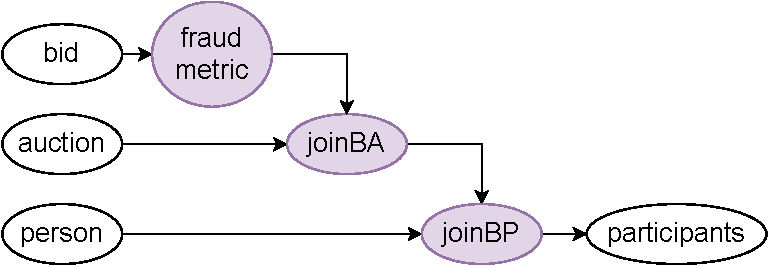
\includegraphics[width=0.6\textwidth]{images/poster.pdf}
    \caption{A possible execution graph for running example.}
    \label{running_example}
\end{figure}


\section{Calco overview}
% We propose to define a distributed dataflow by specifying a set of equivalent execution graphs using a representation called {\em CGraph}.
% An optimal graph can be chosen from this set using a cost-model.

% Since graph operations are user-defined, we need specify their properties manually to define what is the graph equivalency.
% Such specifications we call contracts.
% Input contract specifies requirements that input data flow should satisfy, output contract defines how graph node changes the input data flow.
% Contracts can be defined in different ways, in this paper we describe the trivial definition because of its simplicity.

Graph operations can be user-defined, so we need to add more information about an operation to be aware of the graph equivalency.
Such specifications we call contracts.
Input contract specifies requirements that input data should satisfy, output contract defines how an operation changes the input data.

Input and output data can be described using two sorts of information: attributes that every data element has and properties of such attributes.
Input contract consists of three sets: the required attributes, the required properties, and the prohibited properties.
Output contract consists of two sets: the attributes and the new properties.
Properties are denoted just as strings, like {\em "reliablePerson"} or {\em "popularItem"}.
We say that contracts are satisfied if output contracts match the input contracts within all connected operations in the execution graph.

{\em Environment} is a set of {\em nodes}, annotated with {\em input} and {\em output contracts} (InCont and OutCont).
Nodes can be data sources, one-arity operations, and two-arity operations.

\begin{lstlisting}[language=Haskell]
data Env = Env
  { sources :: Map NodeName OutCont
  , ops1 :: Map NodeName (InCont, OutCont)
  , ops2 :: Map NodeName
                (InCont, InCont, OutCont) }
\end{lstlisting}

Some nodes produce particular side effects that form the result of the running graph (writes data to the storage, displays some statistics on the dashboard, etc.).
Such nodes should exist in all generated execution graphs.
We call the nodes that produce such side effects a {\em graph semantics}.

\begin{lstlisting}[language=Haskell]
type Semantics = Set NodeName
\end{lstlisting}

CGraph is simply a pair of environment and semantics.

\begin{lstlisting}[language=Haskell]
type CGraph = (Env, Semantics)
\end{lstlisting}

Graphs with satisfied contracts that include all semantics nodes form the desired set of equivalent graphs. The implementation of the execution graphs generation algorithm is rather effective despite the brute force approach because graphs that do not satisfy contracts can be ejected. The algorithm is exponential in the size of the semantics set, which is often small enough.

% So using the cost-model we can choose optimal one and run it.
% But having the runtime execution statistics, cost-model can be much more precise.
% Thus we should continuously recompute the execution graphs costs using the updating statistics.
% When the running graph becomes enough less optimal then another graph to compensate the reconfiguration cost, running graph should be dynamically reconfigured.

% \subsection{CGraph}

% Let us define an environment as a set of nodes, annotated with input and output contracts (InCont and OutCont).
% This set consists of the data sources, annotated with OutCont, one arity operations (with one InCont and OutCont) and two arity operations (with two InCont and OutCont).
% Here we limit possible arity of operations for simplicity.

% \begin{lstlisting}[language=Haskell]
% type CSource = OutCont
% type CTfm1 = (InCont, OutCont)
% type CTfm2 = (InCont, InCont, OutCont)

% data Env = Env
%   { sources :: Map NodeName CSource
%   , ops1    :: Map NodeName COp1
%   , ops2    :: Map NodeName COp2 }
% \end{lstlisting}

% Graph gets data from the data sources, transforms it by operations.
% But some of the operation nodes do particular side effects that form result of the graph execution (writes data to the some storage, displays some statistics on the dashboard, etc.).
% Such nodes should exist in all concrete execution graphs that correspond to the given CGraph.
% Let's call the set of the nodes with the such side effects as a graph semantics.
% It will let us to have useless nodes in environment (that are not necessary for graph to have the needed semantics) and reduce the total number of concrete graphs to enumerate.

% \begin{lstlisting}[language=Haskell]
% type Semantics = Set NodeNames
% \end{lstlisting}

% And now we are ready to define CGraph.
% It is simply a pair of environment and semantics.

% \begin{lstlisting}[language=Haskell]
% type CGraph = (Env, Semantics)
% \end{lstlisting}

% \subsection{Data stream state}

% We define here a trivial model of contracts, because the pragmatic model is a bit more complex. (TODO)

% Let's suppose that each element in the data stream is a mapping from attribute names to data (like a row in relational database).
% So the data stream can be described by two sorts of information: attributes that every element has and the properties of the data.
% We can define data stream state as follows:

% \begin{lstlisting}[language=Haskell]
% type Attr = String
% type Prop = String

% data State = State
%   { attrs :: Set Attr
%   , props :: Set Prop }

% empty :: State
% empty = State { attrs = Set.empty
%               , props = Set.empty }

% union :: State -> State -> State
% union s1 s2 = State
%   { attrs s1 `Set.union` attrs s2
%   , props s1 `Set.union` props s2 }
% \end{lstlisting}

% \subsection{Input contracts}

% Input contract can be defined as tuple of three sets:
% \begin{enumerate}
%     \item set of attributes that are required in the input stream,
%     \item set of properties that are required in the input stream,
%     \item set of properties that are prohibited in the input stream.
% \end{enumerate}

% \begin{lstlisting}[language=Haskell]
% data InCont = InCont
%   { attrsI  :: Set Attr
%   , propsI  :: Set Prop
%   , propsI' :: Set Prop }
% \end{lstlisting}

% Operation's input stream state can be matched with the input contract to check if it satisfies that contract.

% \begin{lstlisting}[language=Haskell]
% match :: State -> InCont -> Bool
% match s c =
%      attrsI c `Set.isSubsetOf` attrs s
%   && propsI c `Set.isSubsetOf` props s
%   && propsI' c `Set.disjoint`  props s
% \end{lstlisting}

% \subsection{Output contracts}

% Output contracts can be defined as a tuple of the three sets and one boolean:
% \begin{enumerate}
%     \item set of attributes to be added,
%     \item boolean that is true if an operation is a projection (it removes all attributes that exist in the incoming stream), (TODO can we call this as projection?)
%     \item set of properties to be added,
%     \item set of properties to be deleted.
% \end{enumerate}

% \begin{lstlisting}[language=Haskell]
% data OutCont = OutCont
%   { attrsO  :: Set Attr
%   , delete  :: Bool
%   , propsO  :: Set Prop
%   , propsO' :: Set Prop }
% \end{lstlisting}

% To get the output data stream state of the node, input data stream state should be updated with the output contract of the operation.

% \begin{lstlisting}[language=Haskell]
% update :: State -> OutCont -> State
% update s c = State
%   { attrs = Set.union
%       (attrsO c)
%       (if isProj c then Set.empty
%                    else attrs s)
%   , props = Set.union
%       (propsO c)
%       (props s `Set.difference` propsO' c) }
% \end{lstlisting}

% To get the output data stream state of the data source, empty state should be updated with the source's output contract.

% \begin{lstlisting}[language=Haskell]
% sourceOut :: OutCont -> State
% sourceOut = update State.empty
% \end{lstlisting}

% To get the output data stream state of the one-arity transformation, incoming data stream state should be updated with the transformation's output contract.

% \begin{lstlisting}[language=Haskell]
% tfm1Out :: State -> OutCont -> State
% tfm1Out = update
% \end{lstlisting}

% To get the output data stream state of the two-arity transformation, union of the incoming data streams states should be updated with the transformation's output contract.

% \begin{lstlisting}[language=Haskell]
% tfm2Out :: State -> State
%         -> OutCont -> State
% tfm2Out s1 s2 = update (s1 `State.union` s2)
% \end{lstlisting}

% \subsection{Work scheme}

% All concrete graphs that correspond to the given CGraph can be generated.
% So having the cost function we can choose the most optimal one and run it.
% But having the execution statistics from the runtime, cost function can be much more precise.
% Thus we should continuously recompute the concrete graphs costs using the updating statistics.
% When the running graph becomes enough less optimal then another graph to compensate the reconfiguration cost, running graph should be dynamically reconfigured.

% \subsection{Prototype}

% We have implemented a prototype in Haskell.
% It consists of:
% \begin{enumerate}
%     \item contracts definition and CGraph definition,
%     \item function that checks if a concrete graph corresponds to the given CGraph,
%     \item function that generates all concrete graph that correspond to the given CGraph (runs rather fast because of early enumeration branch truncation),
%     \item set of basic operations that emulate such set of the Apache Beam framework,
%     \item evaluation function that runs the concrete graph.
% \end{enumerate}

% TODO ref https://github.com/flame-stream/halco


\section{Implementation and challenges}
Semantics for the running example consists of the "fraudMetric" and "participants" nodes.
The environment has three sources, two one-arity operations, and two two-arity operations.

For example let us consider contracts of the bid-auction join and the fraud metric.
Join requires "bid.auction" and "auction.id" attributes and sets "joinBA" property:
\begin{lstlisting}[language=Haskell]
( InCont (Set.singleton "bid.auction")
         Set.empty Set.empty
, InCont (Set.singleton "auction.id")
         Set.empty Set.empty
, OutCont Set.empty
          (Set.singleton "joinBA") )
\end{lstlisting}

Fraud metric has one input contract with four alternatives:
only bid attributes
or joined bid and auction attributes
or joined bid and person attributes
or all attributes.

We implemented a graphs generation prototype in Haskell.
Our prototype generates all possible 6 execution graphs corresponding to the CGraph of the running example.

As we mentioned earlier, this work focuses on the problem of equivalent graph generation. The following challenges remain in the adaptation of our technique for end-to-end distributed dataflows optimization:

\textbf{Multicriteria optimization.}
Our framework requires a complex cost model because a user may desire to include some business metrics in the optimization process, e.g., the quality of results or acceptable performance, as we demonstrated in the running example. The planner based on such cost model should use multicriteria optimization that is limitedly studied~\cite{yarygina2014optimizing}.

\textbf{Runtime reconfiguration.}
In batch processing, some systems support dynamic reconfiguration to a new execution graph, e.g., Spark Catalyst~\cite{armbrust2015spark}. Although of efforts on the topic~\cite{grulich2020grizzly}, stream processing systems have a lack of such mechanism for global optimization, e.g., it is unclear how to estimate the cost of reconfiguration in comparison with the potential outcome from the more optimal graph.

\textbf{Improving contracts expressiveness and interoperability.}
Currently, contracts are not convenient enough to use in practice, e.g., if some operations need incoming data not to be filtered, adding new filter property makes a user add it to the prohibited properties set of input contracts of all such operations manually. We also aim to build an automatic contracts generation from popular declarative languages such as SQL.

\section{Conclusion}
In this work, we have outlined two issues regarding the state-of-the-art ways to specify computations in distributed data processing frameworks:
\begin{itemize}
    \item Lack of custom dataflows optimization: modern data processing frameworks consider user-defined operations as black boxes and have limited abilities to optimize execution graphs consisting of such operations.
    \item Lack of cross-domain optimization: if dataflows are defined using various methods, e.g., SQL and graphs, they do not share results and are not optimized together.
\end{itemize}

We have presented a novel framework to specify distributed dataflows.
It is based on the declarative specifications of the graph node properties, which allow us to generate various equivalent graphs for the same task.
We have implemented the prototype of our approach and discussed the challenges we face regarding the selection of the optimal graph, changing the graph in runtime, and the evolution of Calco expressiveness.

\bibliographystyle{splncs04}
\bibliography{bibliography/flame-stream}

\end{document}
